\begin{corrige}{devoir2-0008}
On introduit les nouvelle variables $s=xy$ et $t=y$. Le domaine d'intégration est un rectangle dans le plan $s$-$t$ : $S= [1,2]\times [3,4]$. La fonction à intégrer devient une fonction de la seule variable $s$ : $\sin(xy)=\sin(s)$. Pour compléter l'intégrale il faut encore calculer le déterminant de la matrice Jacobienne de la transformation $(s,t)\mapsto(x,y)$. On écrit $x=s/t$ et $y=t$, donc la matrice Jacobienne est 
\begin{equation}
  \begin{pmatrix}
    \frac{1}{t} & -\frac{s}{t^2}\\
    0 & 1
  \end{pmatrix},
\end{equation}
  et son déterminant est $1/t$. 

On a alors 
\begin{equation}
  \int_1^2\int_3^ 4\frac{\sin(s)}{t}\, dt\, ds=  \int_1^2\sin(s)\,ds\int_3^ 4 \frac{1}{t}dt = \left(-\cos(2)+ \cos(1)\right)\left(\ln(4)-\ln(3)\right).
\end{equation}

\begin{figure}
  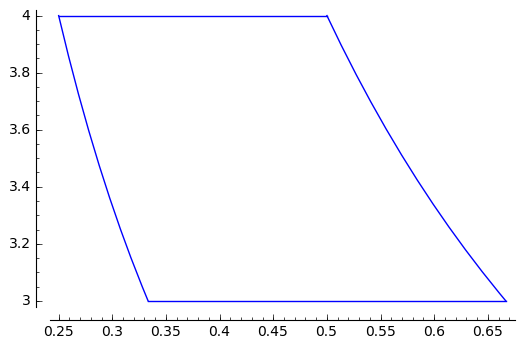
\includegraphics[width=7cm]{Fig_exo7devoir2.png}  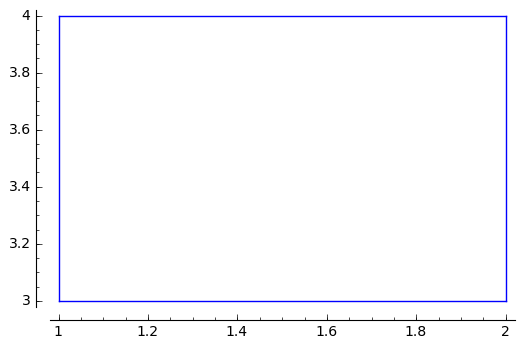
\includegraphics[width=7cm]{Fig_exo7devoir2deuxieme.png}

  \caption{Le domaine d'intégration avant et après le changement de variables}\label{exo7devoir2}
  \end{figure}

\end{corrige}


% Ce \clearpage est là parce que j'ai un «too much floats unprocessed».
% TODO : trouver mieux, et enlever ce \clearpage
\clearpage
